\part{The Foundations}

\chapter{Web Services}\label{chap:web}
In this chapter we lay out foundations for the architecture of Web Services. We
introduce the Resource Oriented Architecture (ROA): a concrete architecture for
Web Service that is constrained by REST. REST builds on the concepts of software
architecture and architectural style; in order to define and understand ROA and
REST it is necessary to define these two concepts first. We introduce the
necessary terminology for Web Services, Software Architecture, REST, and
ROA. Finally, we give a short intro to HTTP caching.

\section{Web Services}
\begin{definition}\label{def:ws}
A Web Service is a software system that support machine-to-machine interaction
over a network via HTTP.
\end{definition}
The definition is a relaxed version, removing the requirements to use
\textit{\gls{gls:wsdl}} and \textit{\gls{gls:soap}}, of the W3C definition
\citep{w3:ws-glos}. In addition, \textit{support} is interchanged with
\textit{designed for} making any Web site accessible by computers also
fall into the category of Web Services.

The Web Services specifically designed for machine-to-machine interaction
typically fall into one of the two categories: RESTful Web Services and Web
Services based on \gls{gls:wsdl}, \gls{gls:soap}, and the \textit{\gls{gls:ws}}
-- known as \textit{\gls{gls:bigws}}. Creating just the smallest Web Service with
Big Web Services demands an excessive amount of plumbing. In a Big Web Service
implementation several things must be defined: the message formats (in SOAP),
data type definition (in XML Schema), and an interface definition (in WSDL). The
plumbing is due to creating a tight contract forcing everything into a standard.

There, however, already exist a standard that has the plumbing in place, Web
Services based on REST with HTTP and Uniform Resource Identifiers (URI). Web
Services based on REST have the great advantage that the means to work with them
are simple. On the client side, the Web Services are accessed with existing
browsers; on the server side, the Web Services are implemented with usual
technologies to create dynamic Web sites. There are scenarios where a RESTful
approach probably wont do the job, such as a distributed transaction protocol
\citep{infoq:rest_ts}. A Web Service under the constraints of REST, however, is
the approach with the lowest entry barrier, and the approach that work with and
not against the nature of the Web, therefore, we decide to travel light, with
REST.

\section{Software architecture and style}
\begin{definition}\label{def:sa}
  A software architecture is the structure(s) ``of a computing system, which
  comprise software elements, the externally visible properties of those
  elements, and the relationships among them'' \citep[p.21]{sa:bass-ch2}.
\end{definition}

The \textit{\gls{gls:defacto}} definition of software architecture,
Definition~\ref{def:sa}, tells that software architecture is first and foremost
an abstraction of the system. The focus is not on internal properties, but on
visible aspects of the system and how the components in the system cooperate.

An important thing about the software architecture is that it is a basis for
archiving quality in the system it pertains to. A software architecture always
facilitates and prohibits different \textit{\gls{gls:qa}}. Ensuring certain
\gls{gls:qa} in the system is done by constraining the architecture in ways known
to affect these; usually facilitated by the use of architectural styles. We
define an architectural style, based on the definition in
\citep[p.24]{sa:bass-ch2}, as follows:
%
\begin{definition}
  An architectural style is a general solution to a problem that describes
  element and relation types and constraints on their use in the software
  architecture.
\end{definition}
%
\textit{The} most important aspect of architectural styles (styles from now) are
that an architecture that satisfy a style exhibit well known \gls{gls:qa} imposed
by the style \citep[p.~25]{sa:bass-ch2}.

\section{REST}
REST is a style designed for systems that handle \textit{\gls{gls:disthyp}}
\citep{rest:Fielding02}. REST defines a set of architectural elements and
constraints on the use of them that facilitate \gls{gls:qa} relevant in a
context of \gls{gls:disthyp}.

REST is the sum of applying several styles for network-based architectures;
Table~\vref{tab:REST} summarizes the styles; the summary includes a short
description of the styles and their effect on a system in terms
of \useGlosentry{gls:qa}{quality attributes}.

The most characteristic style for REST is uniform interface. It defines several
architectural elements and constraints on the use of them. A pivotal
architectural element of the uniform interface is the resource. 

\begin{definition}
A resource is any information that can be named \citep[p.125]{rest:Fielding02}.
\end{definition}
Resources are uniquely identified by a resource identifier. In terms of the Web,
a resource is any information identified by a \textit{\gls{gls:uri}}. Clients that request a
resource get a representation of the resource -- not the resource itself -- in a
format depending on the capabilities of the client. Interaction with resources
are performed through their representations by passing the representations around
in messages and applying the uniform interface on them. Messages are
self-descriptive, which decouples them from the underlying transport layer;
enabling intermediate servers to cache messages, forward messages, etc.

REST stands for Representational State Transfer. The following quote explains the
meaning of it:

\begin{quote}
\footnotesize\itshape
The name ``Representational State Transfer'' is intended to evoke an image of how
a well-designed Web application behaves: a network of Web pages forms a virtual
state machine, allowing a user to progress through the application by selecting a
link or submitting a short data-entry form, with each action resulting in a
transition to the next state of the application by transferring a representation
of that state to the user. \citep[p.116]{rest:Fielding02}
\end{quote}

An architecture that follows the architectural style of REST is called RESTful. A
RESTful architecture exhibits well known \useGlosentry{gls:qa}{quality
attributes} chosen by the designers of REST. Since REST is a model of how the Web
\textit{should} work \citep[p.116]{rest:Fielding02}, a RESTful architecture will
facilitate \useGlosentry{gls:qa}{quality attributes} deemed relevant for the Web.

\section{ROA: A RESTful architecture}
A concrete RESTful architecture is the Resource-Oriented Architecture
\citep[ch.4]{rest:webservice}. ROA is designed specifically for Web
applications; ROA therefore shows how REST is applied using the intrinsic
technologies of the Web, such as HTTP and \gls{gls:uri}. ROA hereby turns
the constraints of REST concrete. By using HTTP many of the styles from
REST are already satisfied:
%%
\begin{itemize}
  \item Client-server: in HTTP only the client is able to make
  requests, while the server is ready to receive them.
  \item Cache: HTTP provides several caching mechanisms, presented in
  Section \ref{sec:caching}.
  \item Code on demand: via HTTP it is possible to transfer
  programs, e.g., JavaScripts or Java applets, to the client and execute them
  locally.
  \item Layered system: HTTP is the medium for client-server
  interaction; what technology, platform,  etc., the server is based on is hidden
  for the client.
\end{itemize}
%%
That many of the styles of REST are already satisfied comes as no surprise: REST
is the style for HTTP and \gls{gls:uri}. ROA ignores the styles a Web application
cannot affect and instead focus on only four styles; each is described in the
following sections.

Throughout this section we examine an existing Web application to give examples
of violations of the styles and their consequences.  The examples
illustrate some of the advantages of a RESTful Web Service by examining the
inverses. The inverses are so common that we denote them as
\textit{\gls{gls:anti_patterns}}. The Web service examined is
\url{rejseplanen.dk}; a journey planning Web Application for bus and train trips in
Denmark.\footnote{\url{rejseplanen.dk} uses HAFAS planning software which is in
use in 16 countries \url{http://www.hacon.de/hafas/}}.

\subsection{Addressability}
Since ROA is based on REST it is centered around the resource architectural
element. In ROA all interesting information provided by the server is a
resource. Resources are identified by a \gls{gls:uri} with a reasonable name
reflecting the concept of the resource \citep[Ch.4]{rest:webservice}. Data on the
server not exposed by a \gls{gls:uri}, are not resources. This
constraint, known in ROA as addressability, gives several advantages:
%%
\begin{itemize}
  \item The provider of data is separated from the consumer of data which
  decouples the application. The decoupling introduces support for arbitrary
  composition of the resources at the client side -- known as mashups.
  \item Caching mechanisms in HTTP have a larger basis to work
  on, because they have a larger contact area with the Web application.
  \item Clients can link to and bookmark specific pages in the Web application.
\end{itemize}
%%
\subsection*{Addressability anti-pattern}
Some Web applications do not expose their interesting information through
\useGlosentry{gls:uri}{URIs}. An example of a web application that violates
addressability is \url{rejseplanen.dk}.

Journey plans from \url{rejseplanen.dk} is shown in
Figure~\ref{fig:rejseplanen_addr}. We arrived at the page after filling out a
search form on the front page, entering the information that we want to go from
Aarhus to Copenhagen, and submitting the form.

%% Behind the scenes, the form submits its values with the
%% \verb|POST| method to \url{http://www.rejseplanen.dk/bin/query.exe/en}.

In the figure we notice that the \gls{gls:uri} of the journey plan page is
unchanged when compared to the main page. This makes it impossible to link to the
journey plan, since the \gls{gls:uri} in the address bar does not reflect the
page currently visited; therefore it is not addressable. The only address ever
exposed in the address bar is the \gls{gls:uri} of the main page. The reason is
that the page uses frames. From a usability perspective, the use of frames was
discouraged already in 1996, because it destroyed addressability
\citep{nielsen:frames}. The addressability violation has a severe impact on the
application: bookmarking the journey plans page is disabled, and the provider and
consumer of data are coupled.

What if the frames are removed? The site expose a search resource, namely the
search engine interface, and not the interesting data behind it. This is contrary
to similar search services, e.g., Google that exposes their data. A Google URI
like \url{http://www.google.com/search?q=addressability} returns a representation
of the directory of the 10 most relevant pages containing the term
addressability. 

%% Creating an addressable Web application, \url{rejseplanen.dk}
%% could expose journey plans resources such as
%% \verb|www.rejseplanen.dk/search?q=aarhus,k�benhavn/|.

%In fact \url{rejseplanen.dk} at their site states wants their web service used by
%both humans and computers \footnote{http://info.rejseplanen.dk/index.php?pageid=208}

%rejseplanen.dk/search?q=aarhus+''my+road'',k�benhav/n

\begin{figure}[htbp]
  \centering
  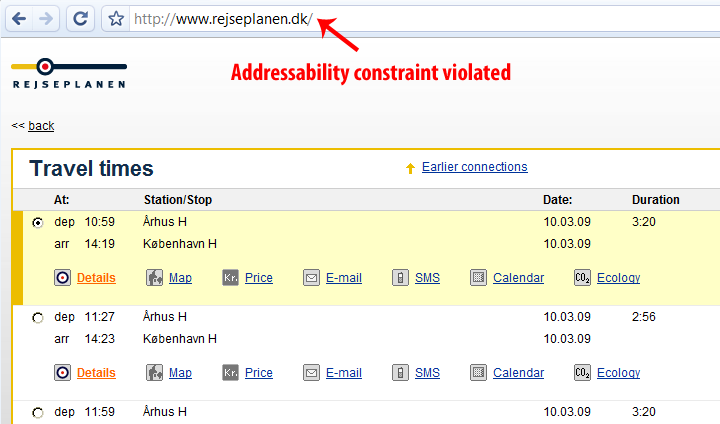
\includegraphics[width=\textwidth]{./Figures/rejseplanen_addr}
  \caption{Addressability violation; [accessed 11-March-2009]} 
  \label{fig:rejseplanen_addr}
\end{figure}

\subsection{Statelessness}
\label{sec:statelessness}
The style of statelessness is enforced in ROA by using HTTP. By design HTTP is
stateless; a workaround is needed to introduce state. An example of this is
cookies \citep[p.145]{rest:Fielding02}. Cookies usually contain a hashed value
referring to a data structure on the server containing
\textit{\gls{gls:appstate}}. Since \gls{gls:appstate} is saved on the server the
stateless style is violated. Cookies used in this way circumvent the quality
advantages introduced by statelessness since servers must use resources to store
client state and replicate state across servers in a clustered environment.
%% http://msdn.microsoft.com/en-us/library/ms525473.aspx

\subsection*{Statelessness anti-pattern}
Many Web applications use cookies to support session state, e.g.,
\url{rejseplanen.dk}. Storing application state for each user demands an
excessive amount of resources on the server. Resources are regained by garbage
collecting session data structures after a short amount of idle time -- typically
less than 20 minutes. Re-accessing a site after the 20 minutes idle time causes
an error because the data structure is removed;
Figure~\ref{fig:rejseplanen_state} shows what happens when we re-access the
journey plans: it causes a failure degrading usability.

In the previous section we criticized the page for violating addressability, but
now it makes sense that the page is not addressable. The statelessness violation
totally removes the option to make the application addressable since all pages
are invalidated after a short amount of time.

\begin{figure}[htbp]
  \centering
  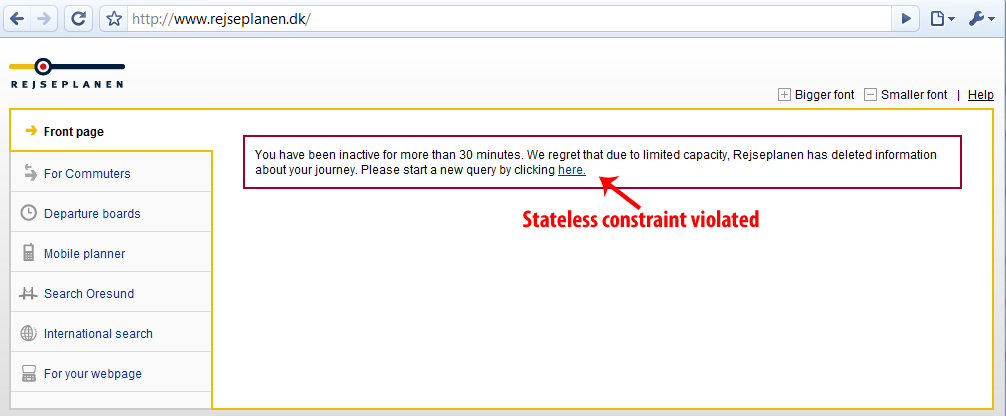
\includegraphics[width=\textwidth]{./Figures/rejseplanen_state}
  \caption{Stateless violation; [re-accessed 11-March-2009]}
  \label{fig:rejseplanen_state}
\end{figure}

\subsection{Uniform interface}\label{sec:ws_uniform_interface}
Clients of RESTful Web Services interact with a resource, through HTTP and the
\gls{gls:uri} of the resource. ROA demands the proper application of the HTTP
methods \citep[ch.4]{rest:webservice}. HTTP defines eight methods that can be
performed on a resource each with well defined semantics \citep{w3:HTTP}. The
semantics of the important methods are given in Table~\ref{tab:HTTP}; it is
indicated whether the methods are idempotent and whether they are safe. Safe and
idempotence are terms defined in \citep{w3:HTTP}. Safe denotes the property that
a method is free of side effects that the user can ``be held accountable
for''. Idempotence denotes the property that ``the side-effects of $N > 0$
identical requests is the same as for a single request.'' The definition of
idempotence is unclear unless side effects are interpreted as the side effects the
user can be held responsible for, e.g., GET is an idempotent operation but in
many cases a GET request changes the server state by writing to the server log,
causing some caching, incrementing a page counter etc. Interpreting side effects
as user responsible side effects allow side effects, such as incrementing a
counter and writing to the log, and does not violate the property of idempotence;
in addition the safe methods become a proper subset of the idempotent methods.

There exist a problem in supporting the uniform interface of HTTP on the
Web. (X)HTML forms only support two HTTP methods: \verb|GET| and \verb|POST|
\citep[sec.17]{w3:HTML}. A workaround is to overload the \verb|POST| method, by adding,
e.g., a \verb|_method| parameter to the query parameters, and route to the
corresponding implementation on the server. To \verb|PUT| or \verb|DELETE| a
resource from a Web browser a form then needs to \verb|POST| to the following
URIs respectively:
%
\begin{verbatim}
  {resource_uri}/?_method=PUT
  {resource_uri}/?_method=DELETE
\end{verbatim}
%

\begin{table}[htbp]
\centering
\setlength\extrarowheight{3pt}
\begin{tabularx}{\textwidth}{l X}
\toprule
HTTP Method    & Semantics\\\midrule
\verb|GET|
               & Retrieve the representation of a resource pointed to by the URI (safe).\\
\verb|HEAD|
               & Same as GET except the response only consist of header fields (safe).\\
\verb|PUT|
               & Create or update the resource identified by the URI in the HTTP message, 
with the representation of the resource located in the body of the HTTP message (idempotent).\\
\verb|DELETE|
               & Delete the resource identified by the URI in the HTTP message (idempotent).\\
\verb|POST|
               & Post the data located in the body of the HTTP message as a new subordinate of %
the resource identified by the URI in the HTTP message (un-idempotent).\\
\bottomrule
\end{tabularx}
\caption{HTTP Methods and their semantics \citep[sec.9]{w3:HTTP}}\label{tab:HTTP}
\end{table}


\subsection*{Uniform interface anti-pattern}
The query interface of \url{rejseplanen.dk}, which consists in an HTML
form, is an example of an illegal use of the HTTP methods in terms of
their semantics. The form uses \verb|POST| to send the query, however, it makes
no sense for the server to create a subordinate resource, in reaction to the
request. 

Browsers notice the use of \verb|POST| and some, e.g., Google Chrome and Safari,
ask for a confirmation when using back / forward buttons, ruining the user
experience, as shown in Figure~\ref{fig:rejseplanen_form}. The warning is
perfectly valid if \verb|POST| is used correctly, namely for posting some data at
the server. In this case, however, it is a misuse of the method; the method is
safe doing nothing besides retrieving data and therefore \verb|GET| should be
used. 

Another unfortunate side effect of the misused \verb|POST| method is that, by
definition, clients must invalidate their cached representation when POST is used
\citep[sec. 13.10]{w3:HTTP}, taking away the advantage of caching.
  
\begin{figure}[htbp]
  \centering
  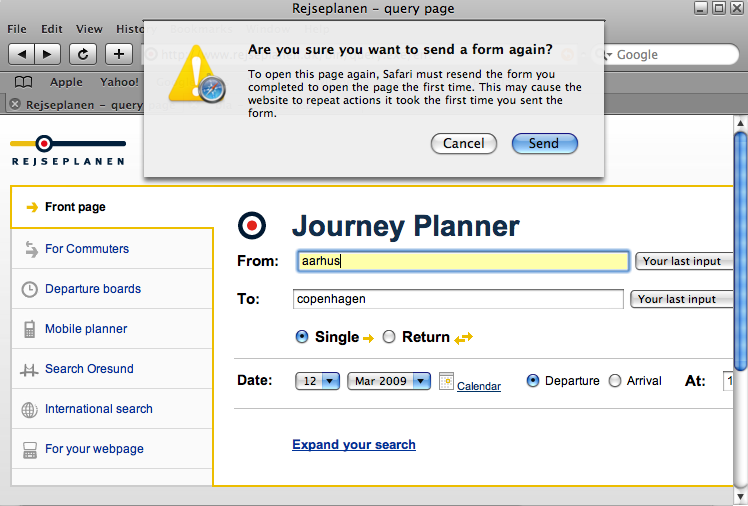
\includegraphics[width=\textwidth]{./Figures/rejseplanen_form_resubmission}
  \caption{Warning message in Safari because of uniform interface violation; [accessed 12-march-2009]}
  \label{fig:rejseplanen_form}
\end{figure}
There are two probable explanations for the illegal use:
%%
\begin{enumerate}
  \item Web crawlers refrain from taking the search link because it uses
    \verb|POST|; reducing use of resources on the server. \url{rejseplanen.dk},
    however, has disabled indexing of all their site, see
    Appendix~\ref{app:fig:rejseplanen_robots}; therefore, resource consumption by
    friendly bots are not a problem.

  \item Internet Explorer imposes a maximum length on URIs to 2,083
    characters\footnote{\url{http://support.microsoft.com/default.aspx?scid=KB;en-us;q208427}}
    although no limit exists in the HTTP specification \citep{w3:HTTP}. The
    limitation does not exist for \verb|POST|, since values in a \verb|POST|
    message does not go into the URI.

    The length of the encoded form is 1562 characters, This is without the
    from-city, the to-city, and a optional via-city. Thus there are over 500
    characters left to encode only 3 places, surely enough, also rendering this
    explanation invalid.
\end{enumerate}
%%
Both reasons are invalid reasons for using \verb|POST|. The explanation probably
lies in \url{rejseplanen.dk} ignoring the HTTP specification, causing unfortunate
side effects for the Web application.

%% http://www.w3.org/Provider/Style/
%% http://www.w3.org/2001/tag/doc/whenToUseGet.html


\subsection{Connectedness}
The style of connectedness states that resources in a Web Service should be
linked together.

\subsection*{Connectedness anti-pattern}
The human Web is a myriad of connected pages in contrast to many Web Services. In
Web Services, connectedness is often forgotten \citep[p.~96]{rest:webservice};
disallowing users ``to progress through the application by selecting a link or
submitting a short data-entry form'' breaking REST. The problem is easily
illustrated by an example: contrast the JSON representation of weather stations in
Listing~\ref{lst:connected_weather_stations} with the representation in
Listing~\ref{lst:ill_weather_stations}.

\begin{lstlisting}[caption=Connected weather stations representation, label=lst:connected_weather_stations]
{
  "next": "/api/weather_stations/?geohash_offset=swgv3sxf003p"}  
  "items": [
    {
      "name": "Skagen", 
      "lat": 57.723952722299998, 
      "lon": 10.5997467041016, 
      "timezone": "Europe/Copenhagen", 
      "type": "DCAWeatherStation", 
      "uri": "/api/weather_stations/dk/skagen/",
      "uri_extern": "http://www.kyst.dk/sw3029.asp", 
      "uri_observations": "/api/weather_stations/dk/skagen/observations/", 
      "uri_scrape": "http://www.kyst.dk/custom_asp/defaultjs.asp?id=3003&targetStation=1100"
    },(...)
  ]
}
\end{lstlisting}

The former is a connected resource containing links to other resources. The
latter is disconnected. A client of the disconnected Web Service must know all
the relevant \gls{gls:uri}s. Clients are bound to break if the Web Service
changes its \gls{gls:uri}s. A Web Service violating connectedness results in a
close coupling between the client and the server.

In a RESTful, i.e., connected Web Service links between resources are available
in the representations, such as \verb|uri_scrape| and \verb|observations| in the
connected example. The added level of indirection decouples clients from the
server since they are now able to use references, instead of direct links, to
resources.

\begin{lstlisting}[caption=Unconnected weather stations representation, label=lst:ill_weather_stations]
{
  "page": 1,
  "has_next": true,
  "items": [
    {
      "name": "Skagen",
      "lat": 57.7239527223,
      "lng": 10.5997467041,
      "type": "DCAWeatherStation", 
      "timezone": "Europe/Copenhagen"
    }
(...)]}
\end{lstlisting}

\section{Caching}\label{sec:caching}
Caching is about one overall thing: reducing the amount of traffic to transfer
over the network. Caching is not a requirement in ROA; however, caching is
pivotal in reducing the latency of Web Services. This section presents the
foundations of HTTP caching.

HTTP caching is a set of mechanisms defined in \citep[Sec. 13]{w3:HTTP} that
indicate to clients and servers which resource representations are cacheable
and when they are stale.

HTTP caching is applied by setting appropriate HTTP headers in the
responses from the server. Advanced clients, such as browsers, perform
caching based on these headers. The content in the caching headers can
be seen as validators; additional client requests trigger the
validators. Only if the validatores are true the client should update
its resource representation.

The caching style of REST (i.e., responses are ``implicitly or explicitly labeled
as cacheable or noncacheable'' \citep[p.121]{rest:Fielding02}) is satisfied in any
HTTP application: if no caching directives is set responses may be cached,
however, it is not expected \citep[sec.13.4]{w3:HTTP}.

There exist three headers to cease explicit control over HTTP
caching:\footnote{We ignore the older caching headers from HTTP 1.0: Expires and
Last-Modified.} \verb|Cache-Control|, \verb|ETag|, and \verb|Vary|; each are
described in the following.

\subsubsection*{Cache-Control}
\verb|Cache-Control| is a header field that controls the valid duration of cached
responses. The field can specify that a cached resource is valid for a relative
time duration. In that time duration all contact with the origin server on
additional requests for the same resource is bypassed.

A header response that defines that the \textit{\gls{gls:ttl}} of a cached
representation is 3600 seconds and applies for all clients, looks like
the following:

\begin{verbatim}
Cache-Control: public, max-age=3600  
\end{verbatim}

A response can also be marked as non-cacheable. The \verb|Cache-Control| field is
the concrete means to do the marking by setting value to \verb|no-cache|. There
is a subtlety in \verb|no-cache|: clients are still allowed to cache responses,
however, before applying the cache they must contact the server to validate that
the cached version corresponds to the server's version. Validation puts forth a
requirement of identifying different versions of a resource, manifested in the
\verb|ETag| field.

\subsubsection*{ETag}
When \gls{gls:ttl} of a representation is overdue the client might still use the
cached version.

\verb|ETag| is a unique identifier attached to resources in requests and
responses. With \verb|ETag| servers validate whether clients' local cached
representation is stale by comparing the \verb|ETag| of the local representation
against the \verb|ETag| of the resource at the server. The server only sends back
a representation upon mismatch of the \verb|ETag|s.

\textit{Note:} Uniqueness of \verb|ETag|s are only in terms of identifiers under
the same URI; therefore, e.g., the last time of modification is a valid \verb|ETag|
value, assuming that no two updates of the same resource can be processed in the
same time frame.

The gain of using \verb|ETag|s is a reduction of the amount of data which are
sent over the network; the total number of requests and responses remain unchanged.

\subsubsection*{Vary}
Since \verb|ETag|s are used to compare a client's representation of a resource
against the \verb|ETag| of the resource at the server, the cache might serve the wrong
representation, but with the correct \verb|ETag|. A common example: given a Web
Service that does \textit{\gls{gls:content_negotiation}} on the type of user
agent, e.g, a mobile user agent or a desktop user agent, a cached response must
only be served to clients of the same type. The \verb|Vary| header field comes to
the rescue and indicates to the client the header fields that can vary the
representations of the resource. The following line indicates how this is
indicated in the HTTP header:

\begin{verbatim}
Vary: User-Agent
\end{verbatim}

\section{Summary}
In this chapter, after having introduced the terms of REST and ROA, we showed
what advantages a RESTful Web Service provides. The advantages were illustrated
by giving examples of a Web Service that violates the styles of REST, and by
discussing the disadvantages the REST violations cause. Finally, we looked at
HTTP caching which is important for increasing the performance of Web Services.

  \begin{sidewaystable}[htbp]
    \centering \setlength\extrarowheight{3pt}
    \begin{tabularx}{\textwidth}{l X X}
    \toprule
Architectural style    & Description        & Effect\\\midrule

Client-server          
               & The system is split up into the provider of a service and the consumer of it.  
               & \textit{Performance} and \textit{modifiability} benefit since separating the concerns makes the server and client simpler and localize changes.\\
Stateless              
               & Client state is disallowed on the server therefore all requests must be standalone.
               & Server \textit{performance} increases, since the server can free resources immediately after requests are processed.\newline
Network \textit{performance} decreases, since messages must be self contained and therefore demands more space.\newline
\textit{Availability} and \textit{modifiability} benefit, since requests can be routed to any server containing the service, 
removing issues of coordination in a clustered environment and losing state on server crashes. \\
Cache                  
               & Results of a request are marked as cacheable or non-cacheable.
               & When caching is applied, \textit{performance} increases due to less network communication and less load on the server. However, the complexity of the application increases, and data staleness also becomes an issue. \\
Uniform interface
               & Components are restricted to a general interface. 
               & \textit{Modifiability} benefit since the overall system architecture is simplified and decoupled. \\
Layered system         
               & The system is split up into hierarchic layers, where layers only use functionality from the layer directly beneath it.
               & \textit{Modifiability} increases, as underlying information is hidden and therefore reduces coupling.\newline
\textit{Performance} decreases since communication must pass through several layers.\\
Code on demand
               & Clients are enabled to download code from the server and execute it locally. 
               & \textit{Performance} increases, since code is executed locally avoiding a round-trip to the server. Load is taken off the server and put on the client. \newline
\textit{Usability} increases since the application reduces latency resulting in a more responsive application.\newline
\textit{Modifiability} benefit since features are easily modified and added to the client \\
    \bottomrule
    \end{tabularx}
  \caption{Architectural Styles of REST (quality attributes are in italics)}\label{tab:REST}
\end{sidewaystable}
